 
\chapter{Ridge Regression}
 

\section{Introduction to ridge regression}

The OLS estimator has many nice properties. For example, Chapter \ref{chapter::gauss-markov} shows that it is BLUE
under the Gauss--Markov model, and Chapter \ref{chapter::normal-linear-model} shows that it follows a Normal distribution that allows for finite-sample exact inference under the Normal linear model. However, it can have the following problems that motivate ridge regression in this chapter. 

The first motivation is quite straightforward. 
From the formula
\[
\hat{\beta}=(X^{\T}X)^{-1}X^{\T}Y,
\]
if the columns of $X$ are highly correlated, then $X^{\T}X$ will
be nearly singular; more extremely, if the number of covariates is larger than the sample size, then $X^{\T}X$ has a rank smaller than
or equal to $n$ and thus is not invertible. So numerically, the OLS
estimator can be unstable due to inverting $X^{\T}X$. Because $X^{\T}X$
must be positive semi-definite, its smallest eigenvalue determines
whether it is invertible or not. \citet{hoerl1970ridge} proposed
the following ridge estimator as a modification of OLS:
\begin{equation}
\hat{\beta}^{\text{ridge}}(\lambda)=(X^{\T}X+\lambda I_{p})^{-1}X^{\T}Y, \qquad(\lambda>0)
\label{eq::ridge-hoerl1970form}
\end{equation}
which involves a positive tuning parameter $\lambda$. 
Because the smallest eigenvalue of $X^{\T}X+\lambda I_{p}$ is larger
than or equal to $\lambda>0$, the ridge estimator is always well
defined. 


Now I turn to the second equivalent motivation. The 
OLS estimator minimizes the residual sum of squares 
$$
\textsc{rss}(b_0,b_1,\ldots,b_p) = 
\sumn(y_{i}-b_{0}-b_{1}x_{i1}-\cdots-b_{p}x_{ip})^{2}.
$$
From Theorem \ref{theorem:varianceinflationfactor} on the variance inflation factor, the variances of the OLS
estimators increase with additional covariates included in the regression,
leading to unnecessarily large estimators by chance. To avoid large OLS coefficients,
we can penalize the residual sum of squares criterion with the squared length of the coefficients\footnote{This is also called the Tikhonov regularization \citep{tikhonov1943stability}. See \citet{bickel2006regularization} for a review of the idea of regularization in statistics.}  
and use
\begin{equation}
\hat{\beta}^{\text{ridge}}(\lambda)=\arg\min_{b_{0},b_{1},\ldots,b_{p}}\left\{ \textsc{rss}(b_0,b_1,\ldots,b_p)+\lambda\sum_{j=1}^{p}b_{j}^{2}\right\} .\label{eq:ridge-definition-1}
\end{equation}
Again in (\ref{eq:ridge-definition-1}), $\lambda $ is a tuning parameter
that ranges from zero to infinity. We first discuss the ridge estimator
with a fixed $\lambda$ and then discuss how to choose it. When $\lambda=0$,
it reduces to OLS; when $\lambda=\infty$, all coefficients must be
zero except that $\hat{\beta}_{0}^{\text{ridge}}(\infty)=\bar{y}$.
With $\lambda \in (0,\infty)$, the ridge coefficients are generally
smaller than the OLS coefficients, and the penalty shrinks the OLS
coefficients toward zero. So the parameter $\lambda$ controls the
magnitudes of the coefficients or the ``complexity'' of the model.
In (\ref{eq:ridge-definition-1}), we only penalize the slope parameters
not the intercept. 


As a dual problem in optimization, we can also
define the ridge estimator as
\begin{align}
\hat{\beta}^{\text{ridge}}(t) & =\arg\min_{b_{0},b_{1},\ldots,b_{p}} \textsc{rss}(b_0,b_1,\ldots,b_p) \nonumber \\
 & \ \textup{s.t. }\sum_{j=1}^{p}b_{j}^{2}\leq t.\label{eq:ridge-definition-2}
\end{align}
Definitions (\ref{eq:ridge-definition-1}) and (\ref{eq:ridge-definition-2})
are equivalent because for a given $\lambda$, we can always find
a $t$ such that the solutions from (\ref{eq:ridge-definition-1})
and (\ref{eq:ridge-definition-2}) are identical. In fact, the corresponding $t$ and $\lambda$ satisfy $t = \|  \hat{\beta}^{\text{ridge}} (\lambda)  \|^2 .$

However, the ridge estimator has an obvious problem: it is not invariant
to linear transformations of $X$. In particular, it is not equivalent
under different scaling of the covariates. Intuitively, the $b_{j}$'s
depend on the scale of $X_{j}$'s, but the penalty term $\sum_{j=1}^{p}b_{j}^{2}$
puts equal weight on each coefficient. A convention in practice is
to standardize the covariates before applying the ridge estimator\footnote{
I choose this standardization because it is the default choice in the function \ri{lm.ridge} in the \ri{R} package \ri{MASS}. 
In practical data analysis, the covariates may have concrete meanings. In those cases, you may not want to scale the covariates in the way as Condition \ref{condition::standardization}. 
However, the discussion below does not rely on the choice of scaling although it requires centering the covariates and outcome. 
}.

\begin{condition}
[standardization]\label{condition::standardization}
The covariates satisfy
\[
n^{-1}\sumn x_{ij}=0,\qquad n^{-1}\sumn x_{ij}^{2}=1,\qquad(j=1,\ldots,p)
\]
and the outcome satisfy $\bar{y} = 0$.
\end{condition}


With all covariates centered at zero, the ridge estimator for
the intercept, given any values of the slopes and the tuning parameter $\lambda$,
equals 
$
\hat{\beta}_{0}^{\text{ridge}}=\bar{y}.
$
So if we center the outcomes at mean zero, then we can drop the intercept
in the ridge estimators defined in (\ref{eq:ridge-definition-1})
and (\ref{eq:ridge-definition-2}). 


For descriptive simplicity, we will assume Condition \ref{condition::standardization} and call it {\it standardization} from now on. This allows us to drop the intercept. Using the matrix form, the ridge estimator minimizes
\[
 (Y-Xb)^{\T}(Y-Xb)+\lambda b^{\T}b,
\]
which is a quadratic function of $b$. From the first order condition, we have
\begin{align*}
%\frac{\partial\textsc{rss}(b,\lambda)}{\partial b} & \mid_{b=\hat{\beta}^{\text{ridge}}(\lambda)}=
&-2X^{\T}\left\{ Y-X\hat{\beta}^{\text{ridge}}(\lambda)\right\} +2\lambda\hat{\beta}^{\text{ridge}}(\lambda)=0\\
\Longrightarrow & \hat{\beta}^{\text{ridge}}(\lambda)=(X^{\T}X+\lambda I_{p})^{-1}X^{\T}Y,
\end{align*}
which coincides with the definition in \eqref{eq::ridge-hoerl1970form}. We also have the second-order condition
\[
%\frac{\partial^{2}\textsc{rss}(b,\lambda)}{\partial b\partial b^{\T}}=
2X^{\T}X+2\lambda I_{p}\succ0,\quad(\lambda>0)
\]
which verifies that the ridge estimator is indeed the minimizer. 
The predicted vector is
$$
\hat{Y}^{\text{ridge}}(\lambda) = X \hat{\beta}^{\text{ridge}}(\lambda)= X (X^{\T}X+\lambda I_{p})^{-1}X^{\T}Y  = H(\lambda) Y,
$$
where $H(\lambda)  =  X (X^{\T}X+\lambda I_{p})^{-1}X^{\T} $ is the hat matrix for ridge regression. When $\lambda = 0$, it reduces to the hat matrix for the OLS; when $\lambda >0$, it is not a projection matrix because $\{  H(\lambda) \} ^2 \neq H(\lambda).$



\section{Ridge regression via the SVD of $X$}







I will focus on the case with $n \geq p$ and relegate the discussion of the case with $n \leq p$ to Problem \ref{hw13::compute-ridge-large-p}. 
To facilitate the presentation, I will use the SVD decomposition of the covariate matrix:
$$
X = UDV^{\T}
$$
where $U \in \mathbb{R}^{n\times p}$ has orthonormal columns such that $U^{\T} U = I_p$, $V \in \mathbb{R}^{p\times p}$ is an orthogonal matrix with $V V^{\T} = V^{\T} V = I_p$, and $D \in \mathbb{R}^{p\times p}$ is a diagonal matrix consisting of the singular values. Figure \ref{fig::svd-X} illustrates this important decomposition. 


\begin{figure}[h]
\centering 
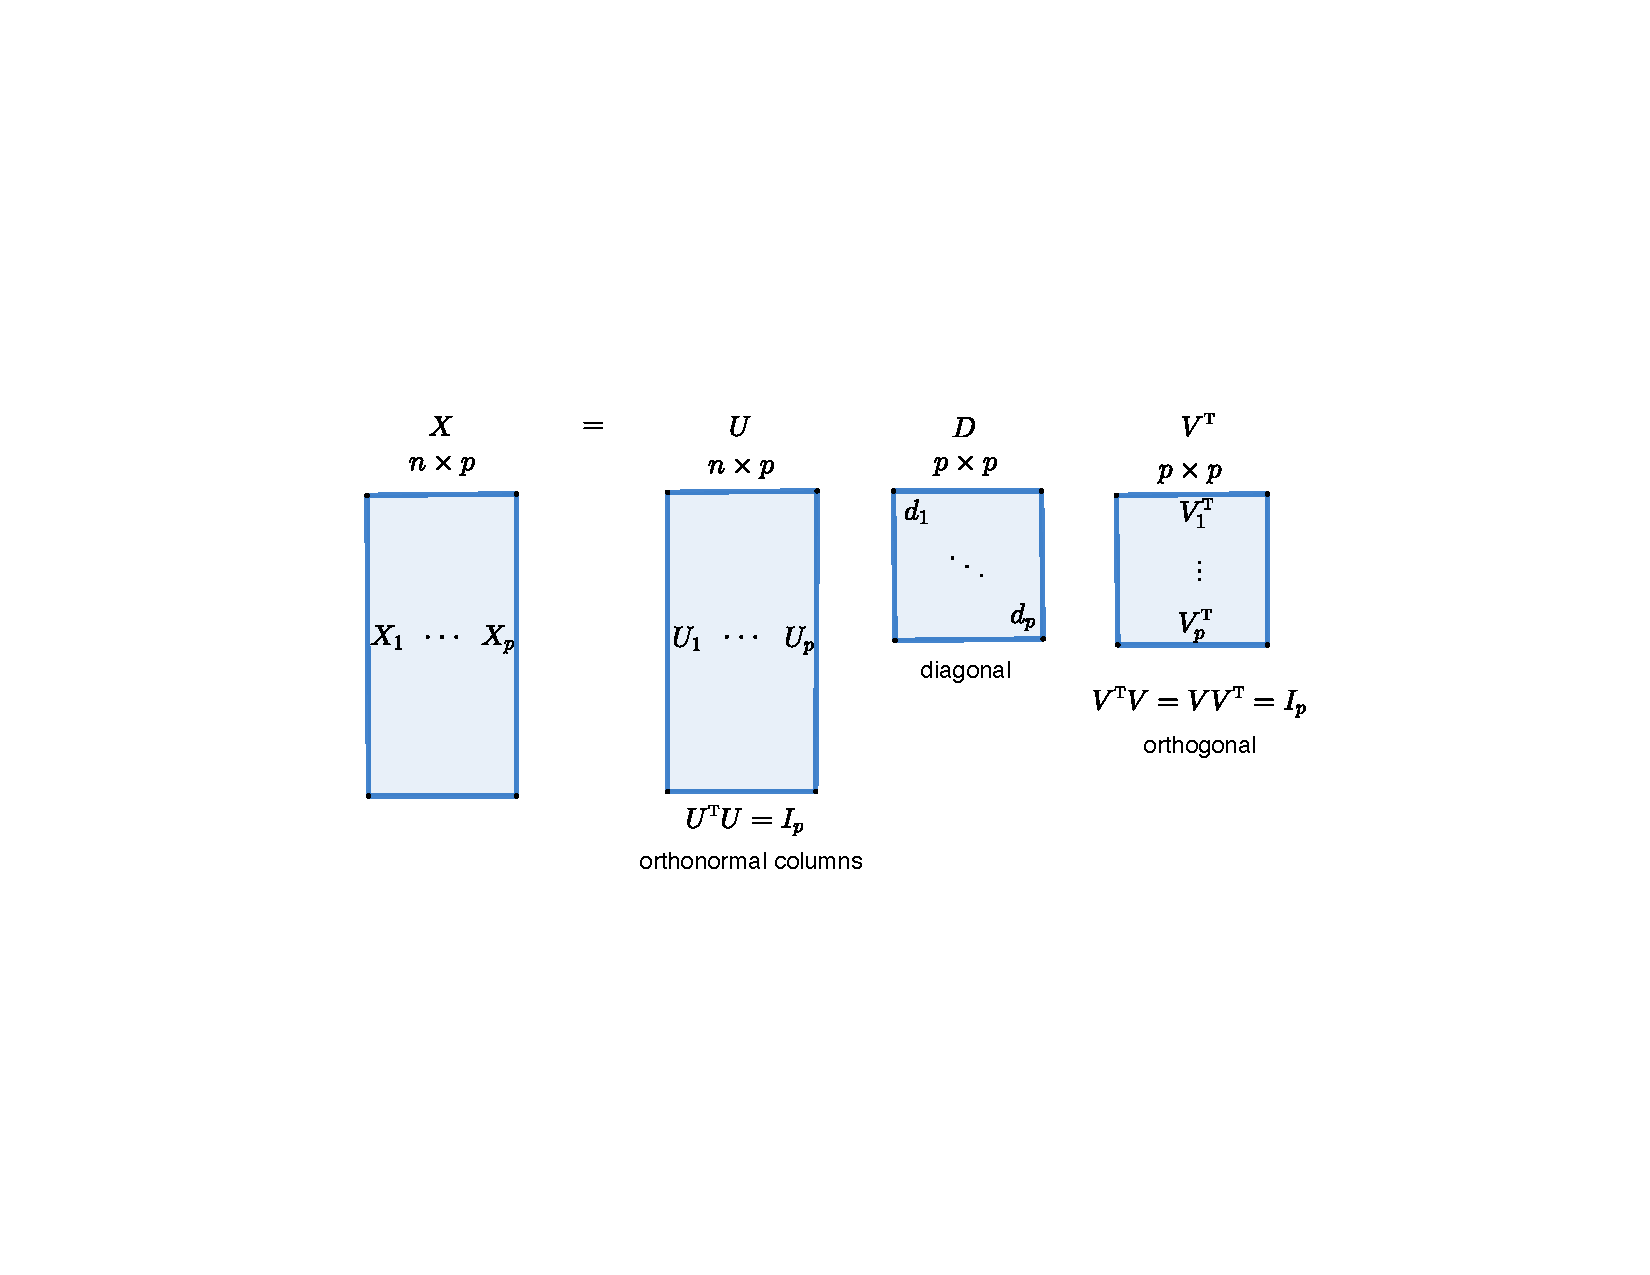
\includegraphics[width = 0.9\textwidth]{figures/svd.pdf}
\caption{SVD of $X$}\label{fig::svd-X}
\end{figure}




The SVD of $X$ implies the eigen-decomposition of $X^{\T} X$:
$$
X^{\T} X = V D^2 V^{\T} 
$$
with eigen-vectors $V_j$ being the column vectors of $V$ and eigen-values $d_j^2$ being the squared singular values.
The following lemma is crucial for simplifying the theory and computation.

\begin{lemma}
\label{lemma::ridge-coefficient}
The ridge coefficient equals
$$
 \hat{\beta}^{\textup{ridge}}(\lambda)  = 
V\textup{diag}\left(  \frac{d_j}{d_j^2 + \lambda }  \right)  U^{\T} Y,
$$
where the diagonal matrix is $p\times p$. 
\end{lemma}


\begin{myproof}{Lemma}{\ref{lemma::ridge-coefficient}}
The ridge coefficient equals
\begin{eqnarray*}
 \hat{\beta}^{\text{ridge}}(\lambda) &=& (X^{\T}X+\lambda I_{p})^{-1}X^{\T}Y \\
 &=& ( VDU^{\T} UD V^{\T}  + \lambda I_p)^{-1} VDU^{\T} Y \\
 &=& V( D^2 + \lambda I_p )^{-1} V^{\T} V D U^{\T} Y\\
 &=& V( D^2 + \lambda I_p )^{-1}   D U^{\T} Y\\
 &=& V\text{diag}\left(  \frac{d_j}{d_j^2 + \lambda }  \right) U^{\T} Y.
\end{eqnarray*}
\end{myproof}





\section{Statistical properties}

The Gauss--Markov theorem shows that the OLS estimator is BLUE under the Gauss--Markov
model: $Y=X\beta+\varepsilon$, where $\varepsilon$ has mean zero
and covariance $\sigma^{2}I_{n}$. Then in what sense, can ridge regression improve OLS? I will discuss the statistical properties of the
ridge estimator under the Gauss--Markov model. 

 


Based on Lemma \ref{lemma::ridge-coefficient}, we can calculate the mean of the ridge estimator:
\begin{eqnarray*}
E\{  \hat{\beta}^{\text{ridge}}(\lambda)\} &=& V\text{diag}\left(  \frac{d_j}{d_j^2 + \lambda }  \right)  U^{\T} X\beta \\
&=&  V\text{diag}\left(  \frac{d_j}{d_j^2 + \lambda }  \right)  U^{\T} UDV^{\T}\beta \\
&=& V\text{diag}\left(  \frac{d_j^2}{d_j^2 + \lambda }  \right) V^{\T}\beta
\end{eqnarray*}
which does not equal $\beta$ in general. So the ridge estimator is biased. We can also calculate the covariance  matrix of the ridge estimator:
\begin{eqnarray*}
\cov\{  \hat{\beta}^{\text{ridge}}(\lambda)\} &=& \sigma^2 V\text{diag}\left(  \frac{d_j}{d_j^2 + \lambda }  \right)  U^{\T}  
U\text{diag}\left(  \frac{d_j}{d_j^2 + \lambda }  \right) V^{\T}  \\
&=&  \sigma^2 V\text{diag}\left(  \frac{d_j^2}{(d_j^2 + \lambda)^2 }  \right)   V^{\T}  . 
\end{eqnarray*}

 
The mean squared error (MSE)
is a measure capturing the bias-variance trade-off:
\[
\textsc{mse}(\lambda)=E\left[\left\{ \hat{\beta}^{\text{ridge}}(\lambda)-\beta\right\} ^{\T}\left\{ \hat{\beta}^{\text{ridge}}(\lambda)-\beta\right\} \right].
\]
Using Theorem \ref{thm::mean-quadratic-form} on the expectation of a quadratic form, we have
\[
\textsc{mse}(\lambda)=\underbrace{    [ E\{  \hat{\beta}^{\text{ridge}}(\lambda)\}  - \beta  ]^{\T} [ E\{  \hat{\beta}^{\text{ridge}}(\lambda)\} - \beta  ]   }_{C_{1}}
+\underbrace{\text{trace}[ \cov\{  \hat{\beta}^{\text{ridge}}(\lambda)\} ]  }_{C_{2}}.
\]
The following theorem simplifies $C_{1}$ and $C_{2}.$ 

 

\begin{theorem}
\label{theorem:bias-variance-tradeoff-ridge} Under  Assumption \ref{assume::gm-model}, the ridge estimator satisfies   
\begin{equation}
C_{1}=\lambda^{2}\sum_{j=1}^{p}\frac{\gamma_{j}^{2}}{( d_j^2 +\lambda)^{2}},\label{eq:term1-ridge-mse}
\end{equation}
where $\gamma=V^{\T}\beta=(\gamma_{1},\ldots,\gamma_{p})^{\T}$ has the $j$th coordinate $\gamma_j = V_j^{\T} \beta$,
and 
\begin{equation}
C_{2}=\sigma^{2}\sum_{j=1}^{p}\frac{ d_j^2 }{( d_j^2 +\lambda)^{2}}.\label{eq:term2-ridge-mse}
\end{equation}
\end{theorem}



\begin{myproof}{Theorem}{\ref{theorem:bias-variance-tradeoff-ridge}}
First, we have 
\begin{eqnarray*}
C_1 &=&     \beta^{\T}      \left\{   V\text{diag}\left(  \frac{d_j^2}{d_j^2 + \lambda }  \right) V^{\T} - I_p   \right\}^2 \beta \\
&=&    \beta^{\T}      V  \text{diag}\left(  \frac{\lambda^2}{ (d_j^2 + \lambda)^2 }  \right)   V^{\T}     \beta \\
&=& \gamma^{\T}  \text{diag}\left(  \frac{\lambda^2}{ (d_j^2 + \lambda)^2 }  \right)   \gamma \\
&=& \lambda^{2}\sum_{j=1}^{p}\frac{\gamma_{j}^{2}}{( d_j^2 +\lambda)^{2}} . 
\end{eqnarray*}

%\begin{align*}
%C_{1} & =\beta^{\T}(S_{\lambda}^{-1}S_0  -I_{p})^{\T}(S_{\lambda}^{-1}S_0-I_{p})\beta\\
% & =\beta^{\T}(V Q_{\lambda}V^{\T}VD^2 V^{\T}-VV^{\T})^{\T}(V Q_{\lambda}V^{\T}VD^2 V^{\T}-VV^{\T})\beta\\
% & =\beta^{\T}V(Q_{\lambda}D^2 -I_{p})^{\T}(Q_{\lambda}D^2 -I_{p})V^{\T}\beta\\
% & =\gamma^{\T}(Q_{\lambda}D^2 -I_{p})^{2}\gamma,
%\end{align*}
%where 
%\[
%(Q_{\lambda}D^2 -I_{p})^{2}=\left(\begin{array}{ccc}
%\frac{ d_i^2 }{ d_i^2 +\lambda}-1\\
% & \ddots\\
% &  & \frac{ d_p^2 }{ d_p^2 +\lambda}-1
%\end{array}\right)^{2}=\left(\begin{array}{ccc}
%\left(\frac{\lambda}{ d_i^2 +\lambda}\right)^{2}\\
% & \ddots\\
% &  & \left(\frac{\lambda}{ d_p^2 +\lambda}\right)^{2}
%\end{array}\right).
%\]
%So (\ref{eq:term1-ridge-mse}) holds. 

Second, we have 
\begin{eqnarray*}
C_2 &=&  \sigma^2 \text{trace} \left( V\text{diag}\left(  \frac{d_j^2}{(d_j^2 + \lambda)^2 }  \right)   V^{\T} \right) \\
&=& \sigma^2 \text{trace} \left( \text{diag}\left(  \frac{d_j^2}{(d_j^2 + \lambda)^2 }  \right ) \right) \\
&=& \sigma^{2}\sum_{j=1}^{p}\frac{ d_j^2 }{( d_j^2 +\lambda)^{2}}. 
\end{eqnarray*}

%\sigma^2 V\text{diag}\left(  \frac{d_j^2}{(d_j^2 + \lambda)^2 }  \right)   V^{\T}
%
%
%\begin{align*}
%C_{2} & =\sigma^{2}\text{trace}\left(S_{\lambda}^{-1}  S_0  S_{\lambda}^{-1}\right)\\
% & =\sigma^{2}\text{trace}\left(V Q_{\lambda}V^{\T}VD^2 V^{\T}V Q_{\lambda}V^{\T}\right)\\
% & =\sigma^{2}\text{trace}\left(V Q_{\lambda}D^2  Q_{\lambda}V^{\T}\right)\\
% & =\sigma^{2}\text{trace}\left(Q_{\lambda}D^2  Q_{\lambda}V^{\T}V\right)\\
% & =\sigma^{2}\text{trace}\left(Q_{\lambda}D^2  Q_{\lambda}\right),
%\end{align*}
%with  
%\[
%Q_{\lambda}D^2  Q_{\lambda}=\left(\begin{array}{ccc}
%\frac{ d_i^2 }{\left( d_i^2 +\lambda\right)^{2}}\\
% & \ddots\\
% &  & \frac{ d_p^2 }{\left( d_p^2 +\lambda\right)^{2}}
%\end{array}\right).
%\]
%so (\ref{eq:term2-ridge-mse}) holds. 
\end{myproof}



Theorem \ref{theorem:bias-variance-tradeoff-ridge} shows the bias-variance trade-off for the ridge estimator. The MSE is 
\begin{eqnarray*}
\textsc{mse}(\lambda) &=& C_{1}+C_{2} \\
&=& \lambda^{2}\sum_{j=1}^{p}\frac{\gamma_{j}^{2}}{( d_j^2 +\lambda)^{2}}+\sigma^{2}\sum_{j=1}^{p}\frac{ d_j^2 }{( d_j^2 +\lambda)^{2}}.
\end{eqnarray*}
When $\lambda=0$, the ridge estimator reduces to the OLS estimator:
the bias is zero and the variance $\sigma^{2}\sum_{j=1}^{p} d_j^{-2}$
dominates. When $\lambda=\infty$, the ridge estimator reduces to
zero: the bias $\sum_{j=1}^{p}\gamma_{j}^{2}$ dominates and the variance
is zero. As we increase $\lambda$ from zero, the bias increases and
the variance decreases. So we face a bias-variance trade-off. 





\section{Selection of the tuning parameter}


\subsection{Based on parameter estimation}
For parameter estimation, we want to choose the $\lambda$ that minimizes the MSE.
So the optimal $\lambda$ must satisfy the following first-order condition:
$$
\frac{\partial\textsc{mse}(\lambda)}{\partial\lambda}  =2\sum_{j=1}^{p}\gamma_{j}^{2}\frac{\lambda}{ d_j^2 +\lambda}\frac{ d_j^2 +\lambda-\lambda}{( d_j^2 +\lambda)^{2}}-2\sigma^{2}\sum_{j=1}^{p}\frac{ d_j^2 }{( d_j^2 +\lambda)^{3}}=0
$$
which is equivalent to
\begin{equation}
\lambda  \sum_{j=1}^{p}\frac{\gamma_{j}^{2} d_j^2 }{( d_j^2 +\lambda)^{3}}=\sigma^{2}\sum_{j=1}^{p}\frac{ d_j^2 }{( d_j^2 +\lambda)^{3}}.\label{eq:optimal-ridge-tuning}
\end{equation}
However, (\ref{eq:optimal-ridge-tuning}) is not directly useful because
we do not know $\gamma$ and $\sigma^{2}$. Three methods below try
to solve (\ref{eq:optimal-ridge-tuning}) approximately. 

\citet{dempster1977simulation} used OLS to construct an unbiased estimator
$\hat{\sigma}^{2}$ and $\hat{\gamma}=V^{\T} \hat{\beta}$, and then
solve $\lambda$ from
\[
\lambda\sum_{j=1}^{p}\frac{\hat{\gamma}_{j}^{2} d_j^2 }{( d_j^2 +\lambda)^{3}}=\hat{\sigma}^{2}\sum_{j=1}^{p}\frac{ d_j^2 }{( d_j^2 +\lambda)^{3}},
\]
which is a nonlinear equation of $\lambda$. 

\citet{hoerl1975ridge} assumed that $X^{\T}X=I_{p}$. Then $ d_j^2 =1\ (j=1,\ldots,p)$
and $\gamma=\beta$, and solve $\lambda$ from
\[
\lambda\sum_{j=1}^{p}\frac{\hat{\beta}_{j}^{2}}{(1+\lambda)^{3}}=\hat{\sigma}^{2}\sum_{j=1}^{p}\frac{1}{(1+\lambda)^{3}},
\]
resulting in
\[
\lambda_{\textsc{hkb}}=p\hat{\sigma}^{2}/\|\hat{\beta}\|^{2}.
\]

\citet{jf1976simulation} used
\[
\lambda_{\textsc{lw}}=p\hat{\sigma}^{2}/\hat{\beta}^{\T}D^2 \hat{\beta}
\]
to weight the $\beta_j$'s based on the eigenvalues of $X^{\T} X$. 

But all these methods require estimating $(\beta,\sigma^{2})$. If
the initial OLS estimator is not reliable, then these estimates of
$\lambda$ are unlikely to be reliable. None of these methods work for the case with $p > n$. 


\subsection{Based on prediction}
For prediction, we need slightly different criteria. 
Without estimating $(\beta,\sigma^{2})$, we can use the leave-one-out cross-validation. The leave-one-out formula for the ridge below is similar to that for OLS.


 
\begin{theorem}\label{thm::looformula-ridge}
Define $\hat{\beta}(\lambda) = (X^{\T} X + \lambda I_p)^{-1} X^{\T} Y$ as the ridge coefficient (dropping the superscript ``ridge'' for simplicity), $\hat{\varepsilon}(\lambda) = Y - X \hat{\beta}(\lambda)$ as the residual vector using the full data, and $ h_{ii} (\lambda) = x_i^{\T} (X^{\T} X + \lambda I_p)^{-1}  x_i$ as the $(i,i)$th diagonal element of $H  (\lambda)  =  X (X^{\T} X + \lambda I_p)^{-1}  X^{\T} $. Define  $\hat{\beta}_{[-i]} (\lambda)$ as the ridge coefficient without observation $i$, and $\hat{\varepsilon}_{[-i]} (\lambda) = y_i - x_i^{\T}  \hat{\beta}_{[-i]} (\lambda)$ as the predicted residual. The leave-one-out formulas for ridge regression are
$$
\hat{\beta}_{[-i]}(\lambda) =  \hat{\beta}(\lambda)  - \{ 1-h_{ii}  (\lambda)  \} ^{-1}  (X^{\T} X + \lambda I_p)^{-1} x_i \hat{\varepsilon}_i(\lambda)
$$
and
$$
\hat{\varepsilon}_{[-i]}(\lambda) = \hat{\varepsilon}_i (\lambda)/ \{  1-h_{ii}  (\lambda) \} .
$$
\end{theorem} 


I leave the proof of Theorem \ref{thm::looformula-ridge} as Problem  \ref{hw13::loo-ridge}. 

By Theorem \ref{thm::looformula-ridge}, the PRESS statistic for ridge is 
$$
\textsc{press}  (\lambda)  = \sumn \left\{   \hat{\varepsilon}_{[-i]} (\lambda) \right \}^2 
= \sumn \frac{   \left\{  \hat{\varepsilon}_i (\lambda) \right\}^2 }{ \{ 1-h_{ii}  (\lambda)  \} ^2 }.
%\cong \frac{  \sumn \left( \hat{\varepsilon}^{\text{ridge}} \right)^2 }{   1 - n^{-1} \text{trace} \{ H(\lambda) \} } .
%=  \frac{  \sumn \left(  \hat{\varepsilon}^{\text{ridge}} \right)^2 }{   1 - n^{-1} \text{trace} \{  X (X^{\T} X + \lambda I_p)^{-1}  X^{\T}\} }. 
$$
 
 
\citet{golub1979generalized} proposed the GCV criterion to simplify the calculation of the PRESS statistic by replacing $h_{ii} (\lambda)$ with their average value $n^{-1} \text{trace}\{ H(\lambda) \}$:
\[
\textsc{gcv}(\lambda)=\frac{\sumn\left\{   \hat{\varepsilon}_i (\lambda)   \right\} ^{2}}{\left[1-n^{-1}\text{trace}\left\{ H(\lambda)\right\} \right]^{2}}.
\]
 
In the \ri{R} package \ri{MASS}, the function \ri{lm.ridge} implements the ridge regression, \ri{kHKB} and \ri{kLW} report two estimators for $\lambda$, and \ri{GCV} contains the GCV values for a sequence of $\lambda$. 
 



 
 
\section{Computation of ridge regression}\label{sec::computation-ridge}
 
 
Lemma \ref{lemma::ridge-coefficient} gives the ridge coefficients. So
 the predicted vector equals
\begin{eqnarray*}
 \hat{Y}(\lambda) &=& X  \hat{\beta}^{\text{ridge}}(\lambda) \\
&=& UDV^{\T} V\text{diag}\left(  \frac{d_j}{d_j^2 + \lambda }  \right)  U^{\T} Y \\
&=& UD \text{diag}\left(  \frac{d_j}{d_j^2 + \lambda }  \right)  U^{\T} Y \\
&=& U \text{diag}\left(  \frac{d_j^2}{d_j^2 + \lambda }  \right)  U^{\T} Y,
\end{eqnarray*}
and the hat matrix equals
\begin{eqnarray*}
H  (\lambda)  = U \text{diag}\left(  \frac{d_j^2}{d_j^2 + \lambda }  \right)   U^{\T}.
\end{eqnarray*}
These formulas allow us to compute the ridge coefficient and predictor vector for many values of $\lambda$ without inverting each $X^{\T} X + \lambda I_p$. 
We have similar formulas for the case with $n<p$; see Problem \ref{hw13::compute-ridge-large-p}.  


A subtle point is due to the standardization of the covariates of the outcome. In \ri{R}, the \ri{lm.ridge} function first computes the ridge coefficient based on the standardized covariates and outcome, and then transforms them back to the original scale. Let $\bar{x}_1,\ldots, \bar{x}_p, \bar{y}$ be the means of the covariates and outcome, and let $\text{sd}_j = \{ n^{-1} \sumn (x_{ij} - \bar{x}_i) ^2 \}^{1/2}$ be the standard deviation of the covariates which are report as \ri{scales} in the output of \ri{lm.ridge}. From the ridge coefficients $\{ \hat{\beta}_1^\text{ridge}(\lambda) ,\ldots,  \hat{\beta}_p^\text{ridge}(\lambda) \}$ based on the standardized variables, we can obtain the predicted values based on the original variables as
$$
\hat{y}_i(\lambda ) - \bar{y} =  \hat{\beta}_1^\text{ridge}(\lambda)  (x_{i1} - \bar{x}_1)/\text{sd}_1 + \cdots +  \hat{\beta}_p^\text{ridge}(\lambda)  (x_{ip} - \bar{x}_p)/\text{sd}_p
$$
or, equivalently,
$$
\hat{y}_i(\lambda )  = \hat\alpha^\text{ridge}(\lambda) 
+  \hat{\beta}_1^\text{ridge}(\lambda) /  \text{sd}_1 \times  x_{i1} + \cdots +  \hat{\beta}_p^\text{ridge}(\lambda)  / \text{sd}_p \times x_{ip}   
$$
where 
$$
\hat\alpha^\text{ridge}(\lambda)  = 
\bar{y} - \hat{\beta}_1^\text{ridge}(\lambda) \bar{x}_1/ \text{sd}_1 -  \cdots - \hat{\beta}_p^\text{ridge}(\lambda) \bar{x}_p/ \text{sd}_p . 
$$



 


\section{Numerical examples}

We can use the following numerical example to illustrate the bias-variance trade-off in selecting $\lambda$ in the ridge. The code is in \ri{code14.5.R}. 



\subsection{Uncorrelated covariates}
 I first simulate data from a Normal linear model with uncorrelated covariates. 
\begin{lstlisting}
library(MASS)
n = 200
p = 100
beta = rep(1/sqrt(p), p) 
sig  = 1/2
X    = matrix(rnorm(n*p), n, p)
X    = scale(X)
X    = X*sqrt(n/(n-1))
Y    = as.vector(X%*%beta + rnorm(n, 0, sig))
\end{lstlisting}


The following code calculates the theoretical bias, variance, and mean squared error, reported in the $(1,1)$th panel of Figure \ref{fig::bias-variance-tradeoff-ridge}.  
 
\begin{lstlisting}
eigenxx = eigen(t(X)%*%X)
xis     = eigenxx$values
gammas  = t(eigenxx$vectors)%*%beta

lambda.seq = seq(0, 70, 0.01)
bias2.seq  = lambda.seq
var.seq    = lambda.seq
mse.seq    = lambda.seq
for(i in 1:length(lambda.seq))
{
	   ll = lambda.seq[i]
	   bias2.seq[i]  = ll^2*sum(gammas^2/(xis + ll)^2)
	   var.seq[i]    = sig^2*sum(xis/(xis + ll)^2)
	   mse.seq[i]    = bias2.seq[i] + var.seq[i]
}
 
y.min = min(bias2.seq, var.seq, mse.seq)
y.max = max(bias2.seq, var.seq, mse.seq)
par(mfrow = c(2, 2))
plot(bias2.seq ~ lambda.seq, type = "l",
     ylim = c(y.min, y.max), 
     xlab = expression(lambda), main = "", 
     ylab = "bias-variance tradeoff", 
     lty = 2, bty = "n")
lines(var.seq ~ lambda.seq, lty = 3)
lines(mse.seq ~ lambda.seq, lwd = 3, lty = 1)
abline(v = lambda.seq[which.min(mse.seq)], 
       lty = 1, col = "grey")
legend("topright", c("bias", "variance", "mse"),
       lty = c(2, 3, 1), lwd = c(1, 1, 4), bty = "n")
\end{lstlisting}


The  $(1,1)$th panel also reported the $\lambda$'s based on different approaches. 

\begin{lstlisting}
ridge.fit = lm.ridge(Y ~ X, lambda = lambda.seq)
abline(v = lambda.seq[which.min(ridge.fit$GCV)], 
       lty = 2, col = "grey")
abline(v = ridge.fit$kHKB, lty = 3, col = "grey")
abline(v = ridge.fit$kLW, lty = 4, col = "grey")
legend("bottomright", 
       c("MSE", "GCV", "HKB", "LW"),
       lty = 1:4, col = "grey", bty = "n")
\end{lstlisting}

I also calculate the prediction error of the ridge estimator in the testing dataset, which follows the same data-generating process as the training dataset. The $(1,2)$th panel of Figure \ref{fig::bias-variance-tradeoff-ridge} shows its relationship with $\lambda$. Overall, GCV, HKB, and LW are similar, but the $\lambda$ selected by the MSE criterion is the worst for prediction. 

\begin{lstlisting}
X.new    = matrix(rnorm(n*p), n, p) 
X.new    = scale(X.new)
X.new    = X.new*matrix(sqrt(n/(n-1)), n, p)
Y.new    = as.vector(X.new%*%beta + rnorm(n, 0, sig))
predict.error = Y.new - X.new%*%ridge.fit$coef
predict.mse   = apply(predict.error^2, 2, mean)
plot(predict.mse ~ lambda.seq, type = "l",
     xlab = expression(lambda),
     ylab = "predicted MSE", bty = "n")
abline(v = lambda.seq[which.min(mse.seq)], 
       lty = 1, col = "grey")
abline(v = lambda.seq[which.min(ridge.fit$GCV)], 
       lty = 2, col = "grey")
abline(v = ridge.fit$kHKB, lty = 3, col = "grey")
abline(v = ridge.fit$kLW, lty = 4, col = "grey")
legend("bottomright", 
       c("MSE", "GCV", "HKB", "LW"),
       lty = 1:4, col = "grey", bty = "n")

mtext("independent covariates", side = 1,
      line = -58, outer = TRUE, font.main = 1, cex=1.5)
\end{lstlisting}


\subsection{Correlated covariates}

I then simulate data from a Normal linear model with correlated covariates. 
\begin{lstlisting}
n = 200
p = 100
beta = rep(1/sqrt(p), p) 
sig  = 1/2
## correlated Normals
X    = matrix(rnorm(n*p), n, p) + rnorm(n, 0, 0.5)
## standardize the covariates
X    = scale(X)
X    = X*matrix(sqrt(n/(n-1)), n, p)
Y    = as.vector(X%*%beta + rnorm(n, 0, sig))
\end{lstlisting}


The second row of Figure \ref{fig::bias-variance-tradeoff-ridge} shows the bias-variance trade-off. Overall, GCV works the best for selecting $\lambda$ for prediction. 

\begin{figure} 
\centering 
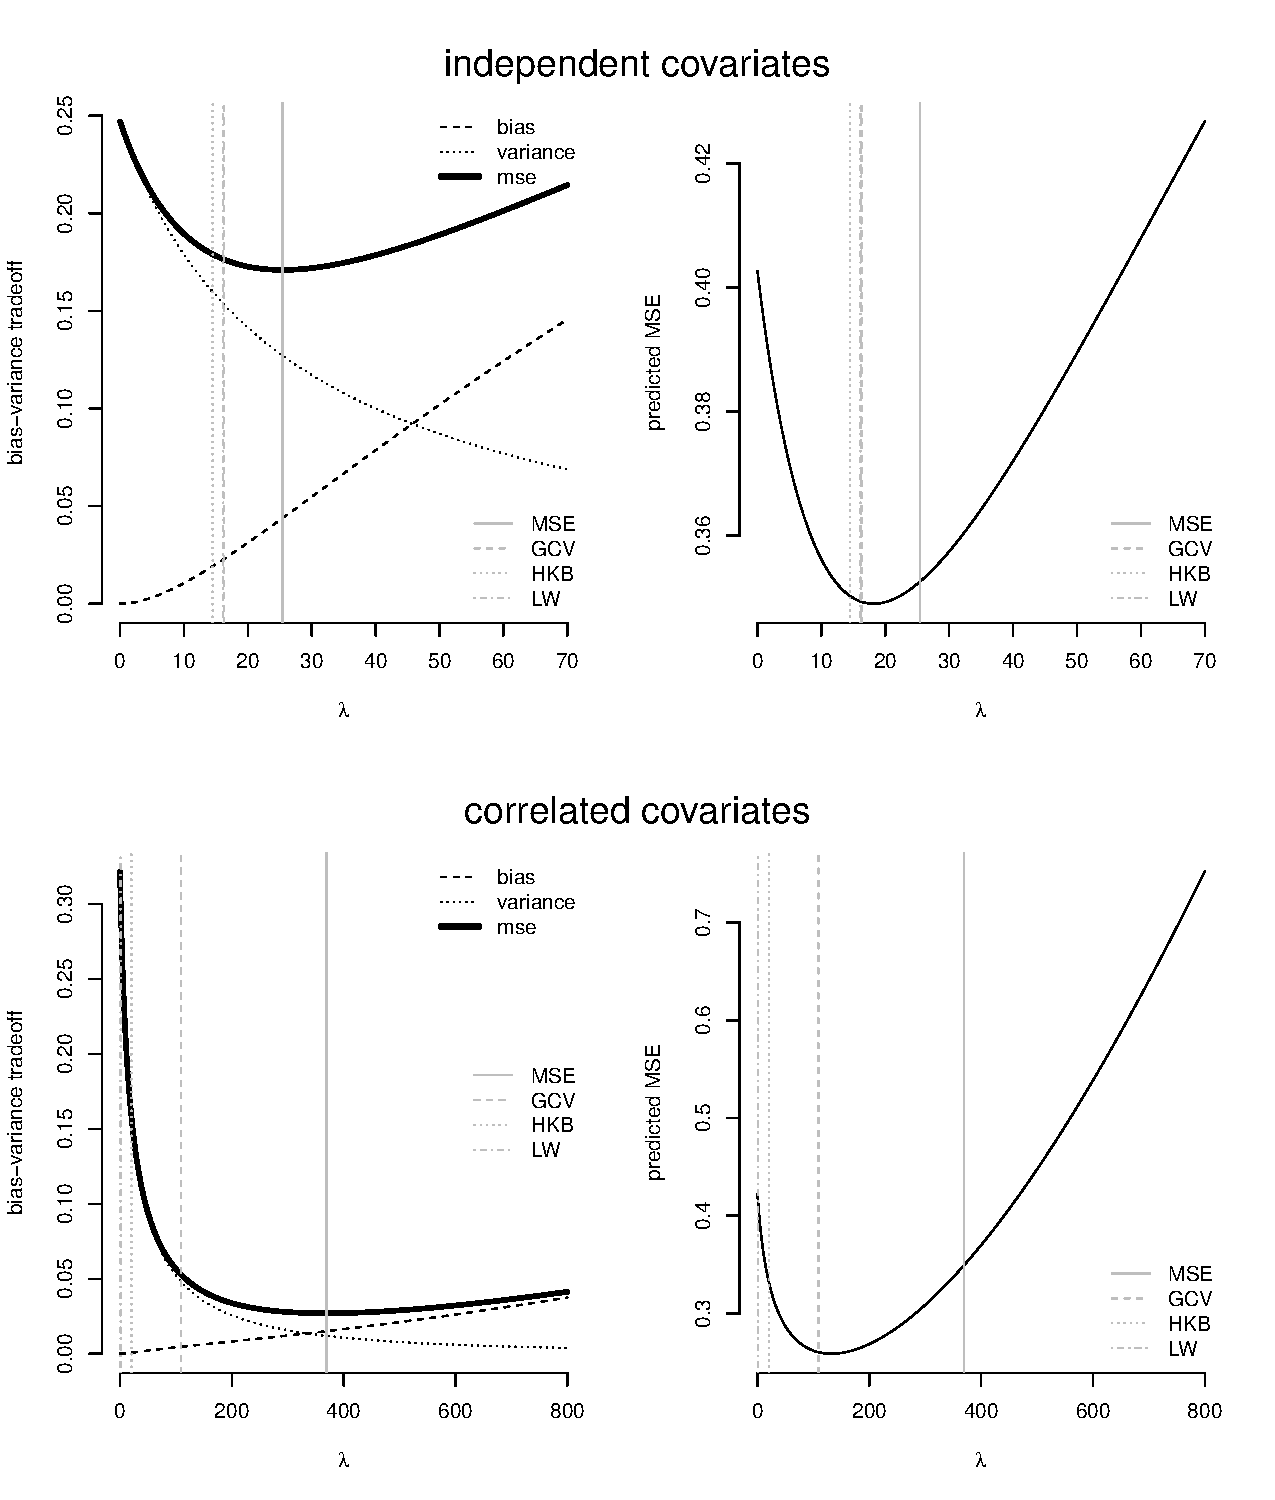
\includegraphics[width = \textwidth]{figures/biasvariancetradeoffridgeplot}
\caption{Bias-variance trade-off in ridge regression}\label{fig::bias-variance-tradeoff-ridge}
\end{figure}




\section{Further commments on OLS, ridge, and PCA}


The SVD of $X$ is closely related to the {\it principal component analysis} (PCA), so is OLS and ridge regression. Assume that the columns of $X$ are centered, so $X^{\T} X = VD^2V^{\T}$ is proportional to the sample covariance matrix of $X$. Assume $d_1 \geq d_2 \geq \cdots$. PCA tries to find linear combinations of the covariate $x_i$ that contain maximal information.   For a vector $v \in \mathbb{R}^p$, the linear combination $v^{\T} x_i $ has sample variance proportional to
$$
Q(v) = 
v^{\T} X^{\T} X v.
$$ 
If we multiply $v$ by a constant $c$, the above sample variance will change by the factor $c^2$. So a meaningful criterion is to maximize $Q(v)$ such that $\|v\| = 1$. This is exactly the setting of Theorem \ref{thm::eigven-max-q}. The maximum value equals $d_1^2$ which is achieved by $V_1$, the first column of $V$. We call
$$
XV_1 = \begin{pmatrix}
x_1^{\T} V_1 \\
\vdots \\
x_n^{\T} V_1
\end{pmatrix}
$$
the first principal component of $X$. Similar to Theorem  \ref{thm::eigven-max-q}, we can further maximize $ Q(v)$ such that $\|v\| = 1$ and $v\perp V_1$, yielding the maximum value $d_2^2$ which is achieved by $V_2$. We call $XV_2$ the second principal component of $X$. By induction, we can define all the $p$ principal components, stacked in the following $n\times p$ matrix: 
$$
(XV_1, \ldots, X V_p) =  XV = UDV^{\T} V = UD.
$$
So $UD$ in the SVD decomposition contains the principal components of $X$. Since $D$ is a diagonal matrix that only changes the scales of the columns of $U$, we also call $U = (U_1, \ldots, U_p)$ the principal components of $X$. They are orthogonal since $U^{\T} U = I_p$. 


Section \ref{sec::computation-ridge} shows that the ridge estimator yields the predicted value
\begin{eqnarray*}
\hat{Y}(\lambda)  &=&  U \text{diag}\left(  \frac{d_j^2}{d_j^2 + \lambda }  \right)  U^{\T} Y \\
&=& \sum_{j=1}^p   \frac{d_j^2}{d_j^2 + \lambda }  \langle U_j , Y\rangle     U_j 
\end{eqnarray*}
where $\langle U_j , Y\rangle = U_j^{\T} Y$ denotes the inner product of vectors $U_j $ and $ Y.$
As a special case with $\lambda = 0$, the OLS estimator yields the predicted value
\begin{eqnarray*}
\hat{Y}    &=& U  U^{\T} Y \\
&=& \sum_{j=1}^p    \langle U_j , Y\rangle     U_j ,
\end{eqnarray*}
which is identical to the predicted value based on OLS of $Y$ on the principal components $U$. Moreover, the principal components in $U$ are orthogonal and have unit length, so the OLS fit of $Y$ on $U$ is equivalent to the component-wise OLS of $Y$ on $U_j$ with coefficient $ \langle U_j , Y\rangle$ $(j=1,\ldots, p)$. So the predicted value based OLS equals a linear combination of the principal components with coefficients  $ \langle U_j , Y\rangle$; the predicted value based on ridge also equals a linear combination of the principal components but the coefficients are shrunk by the factors $d_j^2 / (d_j^2 + \lambda)$. 


When the columns of $X$ are not linearly independent, for example, $p>n$, we cannot run OLS of $Y$ on $X$ or OLS of $Y$ on $U$, but we can still run ridge. Motivated by the formulas above, another approach is to run OLS of $Y$ on the first $p^*$ principal components $ \tilde{U} = ( U_1, \ldots, U_{p^*})$ with $p^* < p$. This is called the {\it principal component regression} (PCR). The predicted value is
\begin{eqnarray*}
\hat{Y} (p^*) &=& (\tilde{U}^{\T} \tilde{U}  )^{-1} \tilde{U} ^{\T} Y \\
&=& \sum_{j=1}^{p^*}    \langle U_j , Y\rangle     U_j ,
\end{eqnarray*}
which truncates the summation in the formula of $\hat{Y} $ based on OLS. 
Compared to the predicted values of OLS and ridge, $\hat{Y} (p^*) $ effectively imposes zero weights on the principal components corresponding to small singular values. It depends on a tuning parameter $p^*$ similar to $\lambda$ in the ridge. Since $p^*$ must be a positive integer and $\lambda$ can be any positive real value, PCR is a discrete procedure while ridge is a continuous procedure.  
 
 


\section{Homework problems}

\paragraph{Ridge coefficient as a posterior mode under a Normal prior}\label{hw13::ridge-bayes}

Assume fixed $X, \sigma^2$ and $\tau^2$. 
Show that if
\[
Y \mid \beta \sim\N(X\beta,\sigma^{2} I_n ),\quad\beta\sim\N(0,\tau^{2}I_{p}),
\]
then the mode of the posterior distribution of $\beta\mid Y$ equals $\hat{\beta}^{\text{ridge}}(\sigma^{2}/\tau^{2})$:
$$
\hat{\beta}^{\text{ridge}}(\sigma^{2}/\tau^{2}) = \arg \max_{\beta} f(  \beta\mid Y  )
$$
where $f(\beta\mid Y)$ is the posterior density of $\beta$ given $Y$. 







\paragraph{Derivative of the MSE}\label{hw13::derivative-of-mse}

Show that 
$$
\frac{\partial\textsc{mse}(\lambda)}{\partial\lambda} \Big |_{\lambda = 0} <0 .
$$

Remark: This result ensures that the ridge estimator must have a smaller MSE than OLS in a neighborhood of $\lambda = 0$, which is coherent with the pattern in Figure \ref{fig::bias-variance-tradeoff-ridge}. 



\paragraph{Ridge and OLS}\label{hw13::ridge-ols}


Show that if  $X$ has linearly independent columns, then
\begin{eqnarray*}
\hat{\beta}^{\text{ridge}}(\lambda) 
&=& (X^{\T} X + \lambda I_p)^{-1} X^{\T} X \hat{\beta} \\
&=& V\text{diag}\left(    \frac{  d_j^2 }{  d_j^2 + \lambda   }  \right) V^{\T}  \hat{\beta}
\end{eqnarray*}
where $\hat{\beta}$ is the OLS coefficient.


\paragraph{Ridge as OLS with augmented data}\label{hw13::ridge-data-aug}

Show that $\hat{\beta}^{\text{ridge}}(\lambda)$ equals the OLS coefficient of $\tilde{Y}$ on $\tilde{X}$ with
augmented data
\[
\tilde{Y}=\left(\begin{array}{c}
Y\\
0_{p}
\end{array}\right),\qquad
\tilde{X}=\left(\begin{array}{c}
X\\
\sqrt{\lambda}I_{p}
\end{array}\right) ,
\]
where $ \tilde{Y}$ is an $n+p$ dimensional vector and $ \tilde{X}$ is an $(n+p)\times p$ matrix. 


Remark: The columns of $\tilde{X}$ must be linearly independent, so the inverse of $\tilde{X}^{\T} \tilde{X}$ always exists. 
This is a theoretical result of the ridge regression. It should not be used for computation especially when $p$ is large. 

\paragraph{Leave-one-out formulas for ridge}\label{hw13::loo-ridge}


Prove Theorem \ref{thm::looformula-ridge}. 


Hint: You can use the result in Problem \ref{hw13::ridge-data-aug} and apply the leave-one-out formulas for OLS in Theorems \ref{thm::leave-one-out-beta} and \ref{theorem:looresidual}. 




\paragraph{Generalized ridge regression}\label{hw13::general-ridge}

Covariates have different importance, so it is reasonable to use different weights in the
penalty term. Find the explicit formula for the ridge regression
with general quadratic penalty:
\[
\arg\min_{b\in\mathbb{R}^{p}}\left\{ (Y-Xb)^{\T}  (Y-Xb) +\lambda b^{\T}Qb\right\} 
\]
where $Q$ is a $p\times p$ positive definite matrix. 





\paragraph{Degrees of freedom of ridge regression}

For a predictor $\hat{Y}$ for $Y$, define the degrees of freedom
of the predictor as $\sumn\cov(y_{i},\hat{y}_{i}) /  \sigma^2 .$ Calculate the
degrees of freedom of ridge regression in terms of the eigenvalues
of $X^{\T}X$. 



\paragraph{Extending the simulation in Figure \ref{fig::bias-variance-tradeoff-ridge}}

Re-run the simulation that generates Figure \ref{fig::bias-variance-tradeoff-ridge}, and report the $\lambda$ selected by \citet{dempster1977simulation}'s method, PRESS, and $K$-fold CV. Extend the simulation to the case with $p>n.$




\paragraph{Unification of OLS, ridge, and PCR}\label{hw13::unification}


We can unify the predicted values of the OLS, ridge, and PCR as
$$
\hat{Y} = \sum_{j=1}^p  s_j  \langle U_j, Y \rangle U_j,
$$
where
$$
s_j  = 
\begin{cases}
1, & \text{OLS}, \\
\frac{  d_j^2 }{   d_j^2 + \lambda  },  & \text{ridge}, \\ 
1(j \leq p^*),  & \text{PCR} .
\end{cases}
$$
Based on the unified formula, show that under Assumption \ref{assume::gm-model}, we have 
$$
E (\hat{Y}  ) = \sum_{j=1}^p s_j d_j \gamma_j U_j
$$
with the $\gamma_j$'s defined in Theorem \ref{theorem:bias-variance-tradeoff-ridge}, and
$$
\cov (\hat{Y}  ) = \sigma^2  \sum_{j=1}^p  s_j^2 U_j U_j^{\T}. 
$$ 




\paragraph{An equivalent form of ridge coefficient}\label{hw13::ridge-equiv-computation}

Show that the ridge coefficient has two equivalent forms: for $\lambda > 0$, 
$$
(X^{\T}X+\lambda I_{p})^{-1}X^{\T}Y = X^{\T} (XX^{\T} + \lambda I_n)^{-1} Y.
$$
 


Remark: This formula has several interesting implications. First, the left-hand side involves inverting a $p\times p$ matrix, and it is more useful when $p<n$; the right-hand side involves inverting an $n\times n$ matrix, so it is more useful when $p>n$. 
Second, from the form on the right-hand side, we can see that the ridge estimator lies in $\mathcal{C}(X^{\T})$, the row space of $X$. That is, the ridge estimator can be written as $X^{\T} \delta $, where $\delta = (XX^{\T} + \lambda I_n)^{-1} Y \in \mathbb{R}^{p}$. This always holds but is particularly interesting in the case with $p>n$ when the row space of $X$ is not the entire $\mathbb{R}^{p}$. 
Third, if $p>n$ and $XX^{\T}$ is invertible, then we can let $\lambda$ go to zero on the right-hand side, yielding
$$
\hat{\beta}^{\text{ridge}}(0) = X^{\T} (XX^{\T}  )^{-1} Y
$$
 which is the minimum norm estimator; see Problem \ref{para::minimum-norm-rols}. Using the definition of the pseudoinverse in Chapter \ref{chapter::linear-algebra}, we can further show that
 $$
 \hat{\beta}^{\text{ridge}}(0) = X^{+} Y. 
 $$
 


\paragraph{Computation of ridge with $n<p$}\label{hw13::compute-ridge-large-p}
When $n<p$, $X$ has singular value decomposition $X = U D V^{\T}$, where $D \in \mathbb{R}^{n\times n}$ is a diagonal matrix containing the singular values, $U\in \mathbb{R}^{n\times n}$ is an orthogonal matrix with $UU^{\T} = U^{\T} U = I_n$, and $V \in \mathbb{R}^{p\times n}$ has orthonormal columns with $V^{\T} V = I_n$. Show that the ridge coefficient, the predicted value, and the hat matrix have the same form as the case with $n>p$.  The only subtle difference is that the diagonal matrices have dimension $n\times n$. 

Remark: The above result also ensures that Theorem \ref{theorem:bias-variance-tradeoff-ridge} holds when $p > n$ if we modify the summation as from $j=1$ to $n$. 






 
\paragraph{Recommended reading}

To celebrate the 50th anniversary of  \citet{hoerl1970ridge}'s paper in {\it Technometrics}, the editor invited Roger W. Hoerl,  the son of Art Hoerl, to review the historical aspects of the original paper, and Trevor Hastie to review the essential role of the idea of ridge regression in data science. See \citet{hoerl2020ridge} and \citet{hastie2020ridge}. 
 
